\section{Reflection}
\label{sec:reflection}

The project ran from the Task 0 proposal in September to this submission on
30 October. Figure~\ref{fig:timeline} places the three tasks, both presentations
and the project's phases on one timeline, beside the commits per day.

\begin{figure}[!htbp]
\centering
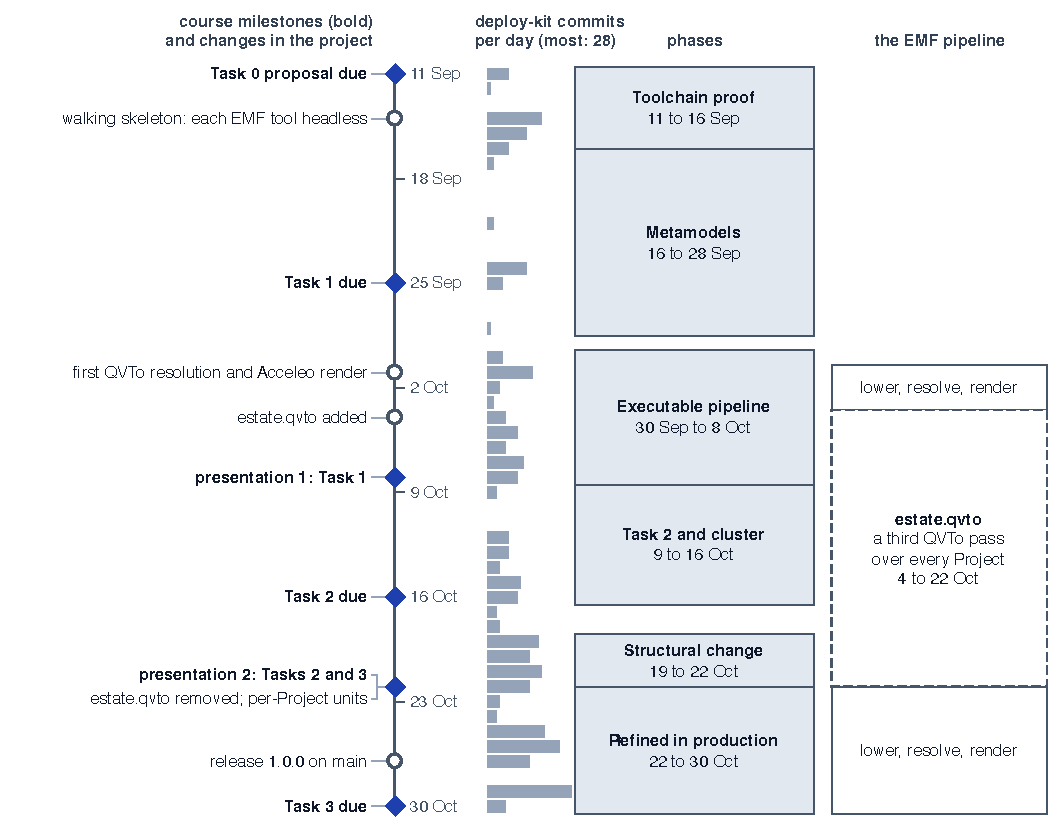
\includegraphics[width=0.78\linewidth, keepaspectratio]{Figures/timeline}
\caption{Project Timeline}
\label{fig:timeline}
\end{figure}
% TODO(verify): Figure 5 (Figures/timeline) must start phase 1 on 14 September (first commit under emf/) and show the Task 1 presentation on 8 October.

\subsection{How the Project Changed Over Time}
\label{sec:timeline-narrative}

The proposal fixed a closed set of inputs, an intermediate Resolved Deployment, a
generated Deliverable Set and two implementations tested against the same examples,
but left the build order open. Priorities shifted through six phases.
\begin{itemize}
\item 14 to 16 September: demonstrating that each tool could run, through the
  headless build, the oracle layout and the parity seam.
\item 16 to 28 September: the metamodels, ending in the Task 1 submission on
  25 September.
\item 30 September to 8 October: the pipeline became executable, with the first
  byte-for-byte Acceleo rendering of \texttt{minimal} on 1 October.
\item 9 to 16 October: the Task 2 report, written after the Task 1 presentation
  on 8 October.
\item 19 to 22 October: the estate pass was removed (Section~\ref{sec:shape-estate});
  the second presentation was on 22 October.
\item 22 to 30 October: the model was refined in production and reached release
  1.0.0; the model-driven implementation adopted each change. In October, the
  repository received 275 commits, 168 of which touched \path{spec/v1}.
\end{itemize}
Three factors drove these shifts: deadlines three weeks apart and then two, cases
surfaced in production, and oracle changes the model-driven implementation had to
follow.

\subsection{What Went Well}
\label{sec:went-well}

\subsubsection{Oracle Parity Across Two Implementations}
\label{sec:went-parity}

Both implementations are held to the same committed oracles, and neither is
generated from the other, so they converged on the same behaviour
(Appendix~\ref{sec:appendix-production}). Section~\ref{sec:oracles} explains the limits of this
evidence.

\subsubsection{Specification and Decisions Before the Reports}
\label{sec:went-spec}

The normative model and the decision records were written before the reports, so
a report could cite the record justifying each decision. The rendered tree of
\texttt{minimal} was committed on 8 September, three weeks before the first
Acceleo template, so it specified the expected output independently of the templates.

\subsubsection{A Headless EMF Toolchain}
\label{sec:went-headless}

Maven with Tycho runs every EMF tool without an IDE, using one dated Eclipse release.
A walking skeleton, metamodel, OCL file and template each ran through its own tool
before substantive content was added. When the Acceleo module arrived on
1 October, subsequent failures therefore concerned content.
% TODO(verify): "every stage run" assumes the CI job runs the full pipeline under mvn verify; confirm against emf/pom.xml.

\subsubsection{Output Tested Against a Live Cluster}
\label{sec:went-cluster}

Applying generated files to a real cluster exposed faults beyond parsers and unit
tests: an immutable Deployment selector, Jobs requiring recreation, and an omitted
Pod Security control. This motivated the server dry-run in Section~\ref{sec:levels}.
% TODO(verify): each cluster fault was found on the cluster rather than in review; the commit subjects support the claim but not the mechanism.

\subsection{What Could Have Been Better}
\label{sec:could-better}

\subsubsection{Structural Changes After Task 2}
\label{sec:late-structure}

The Task 2 report describes three transformations; the estate pass was removed
four days after it was rewritten, so the report is a snapshot of a pipeline that
no longer exists. The appendix records the difference, but the structure should
have been fixed at the Task 2 deadline, with later structural decisions recorded
as changes.

\subsubsection{Acceleo's Whitespace Rules}
\label{sec:whitespace}

Byte comparison directed much of the template work towards presentation. Acceleo 4 strips
a margin from each block-body line; a call repeats the text preceding it on the
line before every output line, so shared templates are written without
indentation (Section~\ref{sec:design}). The \texttt{GENERATED} header, key order
and quoting rule were template decisions made to match the oracle. The effort
concerned output appearance, not transformation semantics.

\subsubsection{Scope}
\label{sec:scope}

The scope was too large for one course. Between 14 September and 30 October, the
repository received 341 commits across the specification, the production
implementation and \path{emf/}, a second implementation of the whole compiler,
and keeping the two level doubled every change. A smaller scope would
have kept the parity, decision records and headless build, held the model at its
Task 1 scope and documented later features as deferred.

\subsubsection{Structural Comparison Came Late}
\label{sec:byte-cost}

For most of the project, output was compared only as bytes: a line diff across
several hundred lines does not distinguish missing keys, extra keys and wrong values.
The structured comparison of Section~\ref{sec:compare-alt} names each difference's
path; adopting it from the start would have saved much debugging.

\subsection{What Was Learned}
\label{sec:learned}

\subsubsection{Decide in the Transformation, Write in the Template}
\label{sec:decide-spell}

Model-to-model transformations make decisions; templates write the results.
When templates derive no values absent from the model, output errors can be traced
either to the model or to target-syntax formatting. The model can then be tested
independently of the template.

\subsubsection{Metamodels as Contracts Between Stages}
\label{sec:contracts}

Typing each stage's model catches errors earlier and makes each stage
replaceable: the estate pass was removed without changing the parser or the
renderer. The cost is that each metamodel changes when its stage does.

\subsubsection{The Cost of Running MDE Tools Without an IDE}
\label{sec:headless-cost}

Most of the effort in model-driven tooling went into running it rather than modelling.
The module's POM changed in at least ten commits, and the indentation rule was established
experimentally. Build configuration and documented tool behaviour therefore deserve
at least as much attention as metamodels.

\subsubsection{Compare Parsed Documents Before Bytes}
\label{sec:structural-oracles}

Oracles should be compared as parsed documents first, then as bytes, and each
stage tested on its own: a failure then names the stage and the field at fault
(Section~\ref{sec:compare-alt}).

% TODO(verify): the Task 0 approval date is recorded only as "September"; confirm the exact date from the course's Canvas record before the hand-in.
